\documentclass[12pt,a4paper]{article} % article, book, report, scrartcl
\usepackage{fullpage}
\usepackage{graphicx}
\usepackage{tabularx,booktabs,dcolumn, longtable, tabu}
\usepackage[english]{babel}
\usepackage[T1]{fontenc}
%\usepackage[ansinew]{inputenc}
\usepackage{ucs}				% Umlaute richtig darstellen 
\usepackage[utf8]{inputenc}		% Umlaute richtig darstellen 
\usepackage{caption}			% für captionof befehle
\usepackage{setspace}			% für 1.5 Zeilenabstand: \onehalfspacing
\usepackage{natbib}
\usepackage{amstext}			% to write text in math equation \text{...}
\usepackage{lscape}				% use landscape environment
\usepackage{fancyvrb}			% to wrap verbatim-code in box
\usepackage{subfigure}
\usepackage{dcolumn}			% for nice regression tables (with texreg in R)
\usepackage{graphicx}
\usepackage[colorlinks=true, linkcolor=black, citecolor=blue]{hyperref}
%\usepackage{subcaption}
\usepackage{todonotes}			% want to ad notes?
\usepackage{mathtools}
\usepackage{savesym}
\usepackage{amsmath}
\savesymbol{iint}
\usepackage{txfonts}
\restoresymbol{TXF}{iint}
\usepackage{amssymb}
\usepackage{pifont} 			% for checkmark sign in tables
% Page settings:
\emergencystretch 1.5em
\widowpenalty=10000
\clubpenalty=10000
\raggedbottom


\title{\begin{large}Networks \& Sports Workshop\end{large}\\[1cm] Social Network Analysis - A Primer for Sport Scientists}
\author{Instructors: Mario Angst and Laurence Brandenberger\\University of Bern and Eawag}
\date{April 19-20, 2018}

\begin{document}
\maketitle

%
\section{Assignment 1 - Handling Network Data}

\subsection{Task 1}

\begin{figure}[!hbt]
\begin{center}
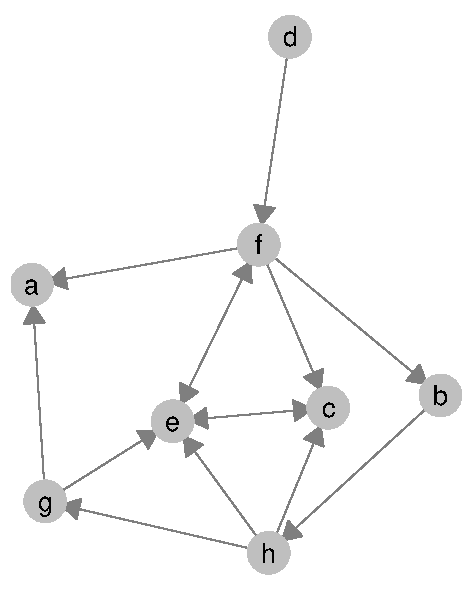
\includegraphics[width = .6\textwidth]{randNW_directed.pdf}
\end{center}
\captionof{figure}{Random directed network}~\label{rdn}
\end{figure}

\begin{enumerate}
	\item Enter the network in Figure \ref{rdn} as an edge list in R.
	\item Convert the edgelist to a matrix.
	\item Plot the network (with the arrows, i.e., directed).
	\item Nodes $a$, $f$, $e$, $c$ are all `smokers', color these nodes blue. Create an attribute-file for your data and add a smoker-variable. Plot the network again. Make sure you include a legend.
\end{enumerate}

\subsection{Task 2}

\begin{enumerate}
	\item Read in the edgelist.
	\item Create an attributes data frame. 
	\item Transform the edgelist into an adjacency matrix.
	\item Create a network object and add at least one attribut to the object.
	\item Plot the network and color nodes with an attribute.
	\item Additional: Size nodes with their indegree-centrality (see help-file for ggnet2).
\end{enumerate}

% 
\clearpage
\newpage
\section{Assignment 2 - Calculating Centrality Scores}

\begin{enumerate}
	\item Using Helga's sports data, set everything up
	\item Compute undirected and directed degree centrality.
	\item Compute closeness and betweenness centrality.
	\item Check for a correlation between a centrality score and an attribute of your choice.
	\item Plot the network again and size the nodes by their betweenness centrality. Interprete the graph.
\end{enumerate}

%
\section{Assignment 3 - Running a Network Autocorrelation Model}

\begin{enumerate}
	\item Prepare Helga's data.
	\item Compute centrality scores.
	\item Compute network autocorrelation terms of your choice (think about your theory first! What do you want to explain?)
	\item Run a simple OLS regression and control for network terms. 
	\item Interpret the results.
	\item Bonus: add an interaction effect and interpret the results.
\end{enumerate}











	
\end{document}